\documentclass[10pt]{beamer}
\usepackage{wrapfig}
\usepackage[export]{adjustbox}
\usepackage[absolute,overlay]{textpos}
\usepackage{amsmath}
\usepackage{ulem}
\usepackage{amsfonts}
\usepackage{tikz}
\usepackage{pgfpages}
\usetikzlibrary{positioning}
\usetheme[
%%% options passed to the outer theme
%    hidetitle,           % hide the (short) title in the sidebar
%    hideauthor,          % hide the (short) author in the sidebar
%    hideinstitute,       % hide the (short) institute in the bottom of the sidebar
%    shownavsym,          % show the navigation symbols
%    width=2cm,           % width of the sidebar (default is 2 cm)
%    hideothersubsections,% hide all subsections but the subsections in the current section
%    hideallsubsections,  % hide all subsections
    left               % right of left position of sidebar (default is right)
%%% options passed to the color theme
%    lightheaderbg,       % use a light header background
  ]{AAUsidebar}

% If you want to change the colors of the various elements in the theme, edit and uncomment the following lines
% Change the bar and sidebar colors:
%\setbeamercolor{AAUsidebar}{fg=red!20,bg=red}
%\setbeamercolor{sidebar}{bg=red!20}
% Change the color of the structural elements:
%\setbeamercolor{structure}{fg=red}
% Change the frame title text color:
%\setbeamercolor{frametitle}{fg=blue}
% Change the normal text color background:
%\setbeamercolor{normal text}{bg=gray!10}
% ... and you can of course change a lot more - see the beamer user manual.


\usepackage[utf8]{inputenc}
\usepackage[danish]{babel}
\usepackage[T1]{fontenc}
% Or whatever. Note that the encoding and the font should match. If T1
% does not look nice, try deleting the line with the fontenc.
\usepackage{helvet}
\usepackage{listings}
\usepackage{tikz}
\usepackage{caption}
\usepackage{subfigure}
\usepackage{graphicx}
\usetikzlibrary{matrix,backgrounds}
% colored hyperlinks
\newcommand{\chref}[2]{%
  \href{#1}{{\usebeamercolor[bg]{AAUsidebar}#2}}%
}

\newenvironment{proenv}{\only{\setbeamercolor{local structure}{fg=green}}}{}
\newenvironment{conenv}{\only{\setbeamercolor{local structure}{fg=red}}}{}

\title[Hiding in Plain Sight]% optional, use only with long paper titles
{Hiding in Plain Sight}

\subtitle{Using Graph Theory to Hide Data in JPEG Images}  % could also be a conference name

\date{30 Juni 2016}

\author[DAT2-A423] % optional, use only with lots of authors
{
  DAT2-423\\
  \href{mailto:dat2a423@student.aau.dk}{{\tt dat2a423@student.aau.dk}}
}
% - Give the names in the same order as they appear in the paper.
% - Use the \inst{?} command only if the authors have different
%   affiliation. See the beamer manual for an example

\institute[
%  {\includegraphics[scale=0.2]{aau_segl}}\\ %insert a company, department or university logo
  Datalogi\\
  Aalborg Universitet\\
  Danmark
] % optional - is placed in the bottom of the sidebar on every slide
{% is placed on the title page
  Datalogi\\
  Aalborg Universitet\\
  Danmark
  
  %there must be an empty line above this line - otherwise some unwanted space is added between the university and the country (I do not know why;( )
}


% specify a logo on the titlepage (you can specify additional logos an include them in 
% institute command below
\pgfdeclareimage[height=1.5cm]{titlepagelogo}{AAUgraphics/aau_logo_new} % placed on the title page
%\pgfdeclareimage[height=1.5cm]{titlepagelogo2}{graphics/aau_logo_new} % placed on the title page
\titlegraphic{% is placed on the bottom of the title page
  \pgfuseimage{titlepagelogo}
%  \hspace{1cm}\pgfuseimage{titlepagelogo2}
}


\begin{document}
% the titlepage
{\aauwavesbg%
\begin{frame}[plain,noframenumbering] % the plain option removes the sidebar and header from the title page
  \titlepage
\end{frame}}
%%%%%%%%%%%%%%%%

% TOC
\begin{frame}{Agenda}{}
\tableofcontents
\end{frame}

% -*- root: ../Presentation.tex -*-
\section{Optimeringer}
\begin{frame}{Optimeringer}{}
		\begin{figure}[!H]
			\centering
			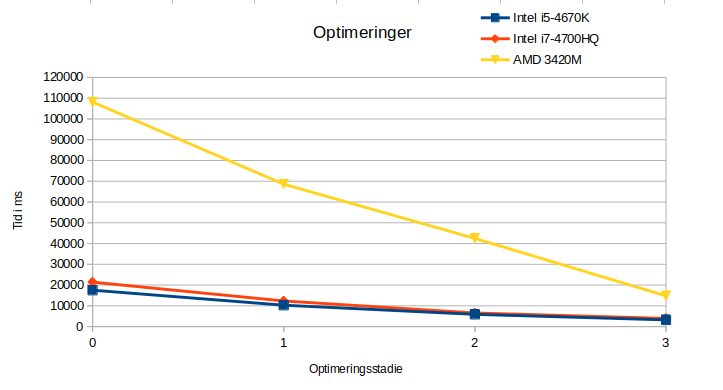
\includegraphics[width=1\textwidth]{Jacob/Selection_744.png}
	\end{figure}
\note{
	1:
	\begin{itemize}
		\item Loop logic conditions beregning flyttet ud af loop
		\item padcover image kører kun når det er nødvendigt
		\item padcoverimage bruger ikke getpixel/setpixel
	\end{itemize}

	2:
	\begin{itemize}
		\item splitToChannels bruger ikke getPixel
	\end{itemize}

	3:
	\begin{itemize}
		\item Multithreading
	\end{itemize}
}
\end{frame}
% -*- root: ../Presentation.tex -*-
\section{Programdemo}
%PNG SECTION
\begin{frame}{Programdemo}{}
	
\end{frame}
% -*- root: ../Presentation.tex -*-
\section{Forbedringer}
\begin{frame}{Forbedringer til programmet}{}
	Problemer vi ville løse:
	\begin{itemize}
		\item Primitiv tilgang til \lstinline|Graph| klassens opbygning
		\item Megen funktionalitet gemt i \lstinline|JPEGImage| klassen
	\end{itemize}
\end{frame}

\subsection{Ændringer til \lstinline|Graph|}
\begin{frame}{Ændringer til \lstinline|Graph|}{}
	3 forskellige måder at opbygge en graf:
	\begin{enumerate}
		\item Liste af Vertices og Edges\uncover<2-2>{\textcolor{red}{$\leftarrow$}}
		\item Naboliste (Adjacency List)\uncover<3-3>{\textcolor{red}{$\leftarrow$}}
		\item Nabomatrix (Adjacency Matrix)
	\end{enumerate}
\note<.-> {
	I afsnit 3.3  diskuteres forskellige fremstillinger. Vi bruger den simple, men beskriver adjancency listen som værende en god ide.

	Vi havde et ønske om at benytte den
}
\end{frame}

\begin{frame}{Fordel ved naboliste}{}

\includegraphics[width=\textwidth]{figures/graphLists.png}
\note<.-> {
	(1)
	For at slette en kant skal vi loope igennem alle vores kanter, og kun slette dem vi skal bruge.
	Resulterer i mange spildte operationer

	(2)
	Vi skal kun loope igennem de kanter der bliver peget på af edges i naboerne til en vertex
}
\end{frame}



\begin{frame}[fragile]{Svaret er...}{}
\lstinline|GraphEncoder|
\begin{itemize}
	\item Håndterer alt graf-enkodning
	\item En generel løsning fremfor specialsyet til JPEG
	\item Maksimerer data-hiding og testabilitet
\end{itemize}

\only<1-1> {
	\lstinputlisting[breaklines=true,basicstyle=\tiny,frame=single]{Mathias/code1.cs}
}
\only<2-2> {
	\lstinputlisting[breaklines=true,basicstyle=\tiny,frame=single]{Mathias/code2.cs}
}
\note<.->{
	Vi kan gemme alt graf væk fra JPEG. Det er kun grafen selv der behøver at kende til det.

	Dette betyder at løsningen kan fungere på ``alle'' tal. Ikke kun AC koefficienter. GraphEncoder er ligeglad hvor tallene kommer fra

	Vi kan gøre løsningen mere fleksibel ved hjælp af interfaces

	Forskellige typer af graffremstillinger kunne skiftes ud på runtime eller når et nyt bliver lavet
}
\end{frame}
% -*- root: ../Presentation.tex -*-
\section{Status}
\begin{frame}{Status}{}
\begin{figure}
\centering     %%% not \center
\subfigure[Grænseværdier på gamle program]{\label{fig:a}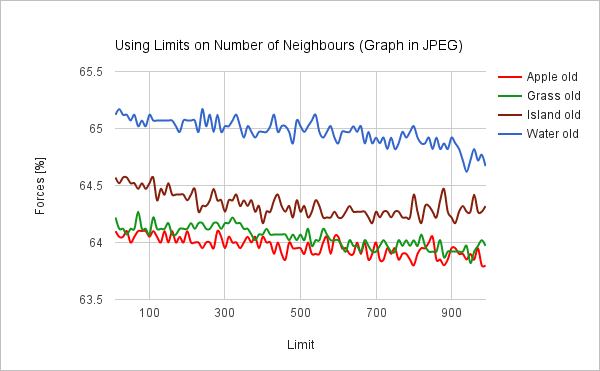
\includegraphics[width=.5\textwidth]{figures/graphOld.png}}
\subfigure[Grænseværdier på nye program]{\label{fig:b}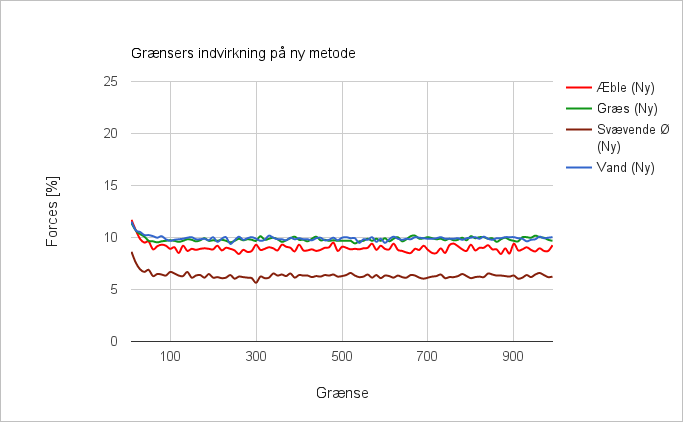
\includegraphics[width=.5\textwidth]{figures/graphNew.png}}
\caption{my caption}
\end{figure}
\end{frame}
\begin{frame}{Status}{}
\begin{figure}
\centering     %%% not \center
\subfigure[]{\label{fig:a}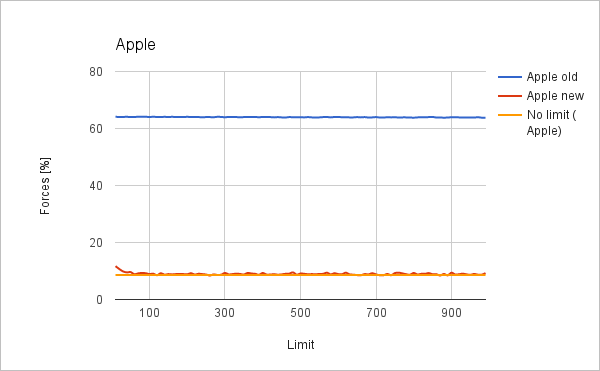
\includegraphics[width=.4\textwidth]{figures/graphApple.png}}
\subfigure[]{\label{fig:b}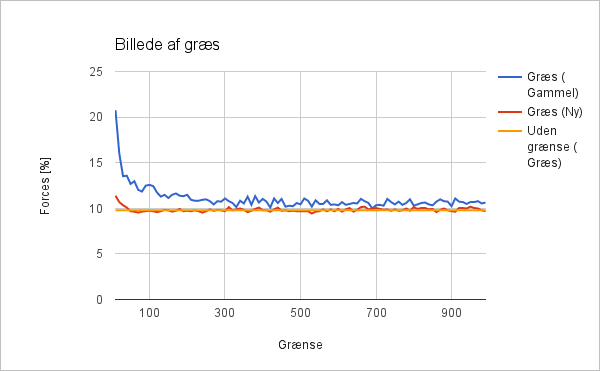
\includegraphics[width=.4\textwidth]{figures/graphGrass.png}}
\subfigure[]{\label{fig:a}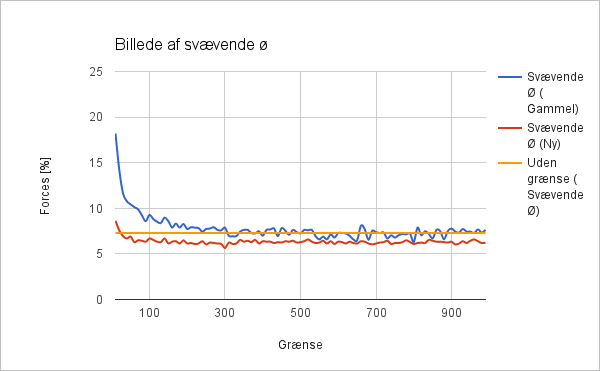
\includegraphics[width=.4\textwidth]{figures/graphIsland.png}}
\subfigure[]{\label{fig:b}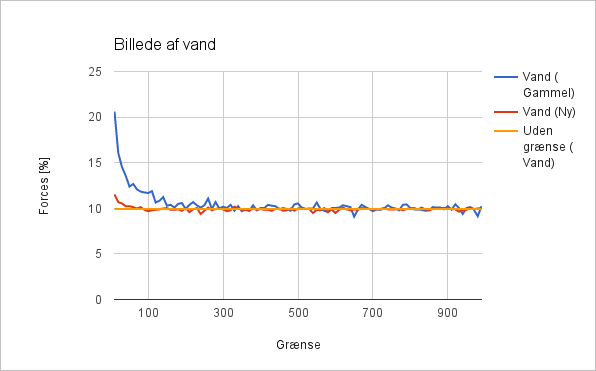
\includegraphics[width=.4\textwidth]{figures/graphWater.png}}
\caption{Sammenligning af grænseværdier}
\label{fig:limits}
\end{figure}
\end{frame}

\begin{frame}{Status}{}
\begin{figure}
\centering     %%% not \center
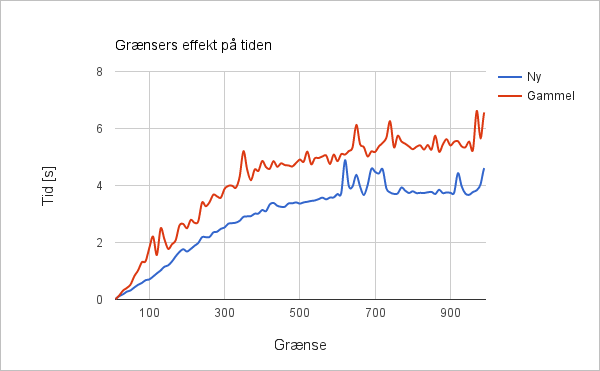
\includegraphics[width=.6\textwidth]{figures/graphTime.png}
\caption{Effekten fra grænseværdier på tiden}
\label{fig:limits}
\end{figure}
\end{frame}
    % Intro, problemanalyse (sociale medier & problemformulering)
% -*- root: ../Presentation.tex -*-
\section{Optimeringer}
\begin{frame}{Optimeringer}{}
		\begin{figure}[!H]
			\centering
			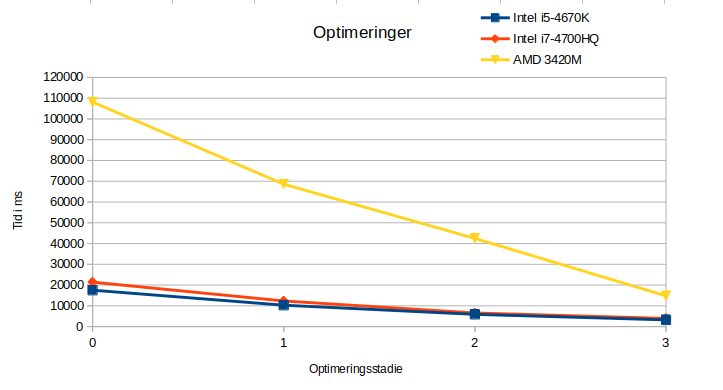
\includegraphics[width=1\textwidth]{Jacob/Selection_744.png}
	\end{figure}
\note{
	1:
	\begin{itemize}
		\item Loop logic conditions beregning flyttet ud af loop
		\item padcover image kører kun når det er nødvendigt
		\item padcoverimage bruger ikke getpixel/setpixel
	\end{itemize}

	2:
	\begin{itemize}
		\item splitToChannels bruger ikke getPixel
	\end{itemize}

	3:
	\begin{itemize}
		\item Multithreading
	\end{itemize}
}
\end{frame}
% -*- root: ../Presentation.tex -*-
\section{Programdemo}
%PNG SECTION
\begin{frame}{Programdemo}{}
	
\end{frame}
% -*- root: ../Presentation.tex -*-
\section{Forbedringer}
\begin{frame}{Forbedringer til programmet}{}
	Problemer vi ville løse:
	\begin{itemize}
		\item Primitiv tilgang til \lstinline|Graph| klassens opbygning
		\item Megen funktionalitet gemt i \lstinline|JPEGImage| klassen
	\end{itemize}
\end{frame}

\subsection{Ændringer til \lstinline|Graph|}
\begin{frame}{Ændringer til \lstinline|Graph|}{}
	3 forskellige måder at opbygge en graf:
	\begin{enumerate}
		\item Liste af Vertices og Edges\uncover<2-2>{\textcolor{red}{$\leftarrow$}}
		\item Naboliste (Adjacency List)\uncover<3-3>{\textcolor{red}{$\leftarrow$}}
		\item Nabomatrix (Adjacency Matrix)
	\end{enumerate}
\note<.-> {
	I afsnit 3.3  diskuteres forskellige fremstillinger. Vi bruger den simple, men beskriver adjancency listen som værende en god ide.

	Vi havde et ønske om at benytte den
}
\end{frame}

\begin{frame}{Fordel ved naboliste}{}

\includegraphics[width=\textwidth]{figures/graphLists.png}
\note<.-> {
	(1)
	For at slette en kant skal vi loope igennem alle vores kanter, og kun slette dem vi skal bruge.
	Resulterer i mange spildte operationer

	(2)
	Vi skal kun loope igennem de kanter der bliver peget på af edges i naboerne til en vertex
}
\end{frame}



\begin{frame}[fragile]{Svaret er...}{}
\lstinline|GraphEncoder|
\begin{itemize}
	\item Håndterer alt graf-enkodning
	\item En generel løsning fremfor specialsyet til JPEG
	\item Maksimerer data-hiding og testabilitet
\end{itemize}

\only<1-1> {
	\lstinputlisting[breaklines=true,basicstyle=\tiny,frame=single]{Mathias/code1.cs}
}
\only<2-2> {
	\lstinputlisting[breaklines=true,basicstyle=\tiny,frame=single]{Mathias/code2.cs}
}
\note<.->{
	Vi kan gemme alt graf væk fra JPEG. Det er kun grafen selv der behøver at kende til det.

	Dette betyder at løsningen kan fungere på ``alle'' tal. Ikke kun AC koefficienter. GraphEncoder er ligeglad hvor tallene kommer fra

	Vi kan gøre løsningen mere fleksibel ved hjælp af interfaces

	Forskellige typer af graffremstillinger kunne skiftes ud på runtime eller når et nyt bliver lavet
}
\end{frame}
% -*- root: ../Presentation.tex -*-
\section{Status}
\begin{frame}{Status}{}
\begin{figure}
\centering     %%% not \center
\subfigure[Grænseværdier på gamle program]{\label{fig:a}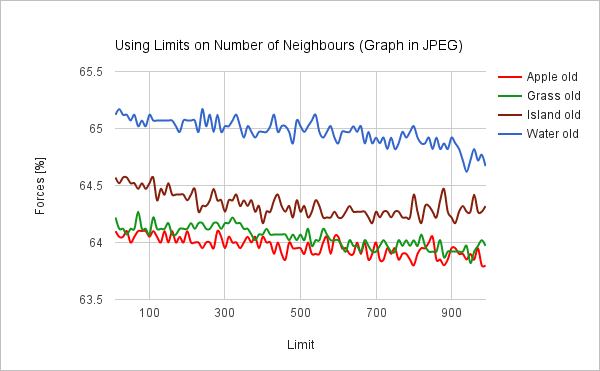
\includegraphics[width=.5\textwidth]{figures/graphOld.png}}
\subfigure[Grænseværdier på nye program]{\label{fig:b}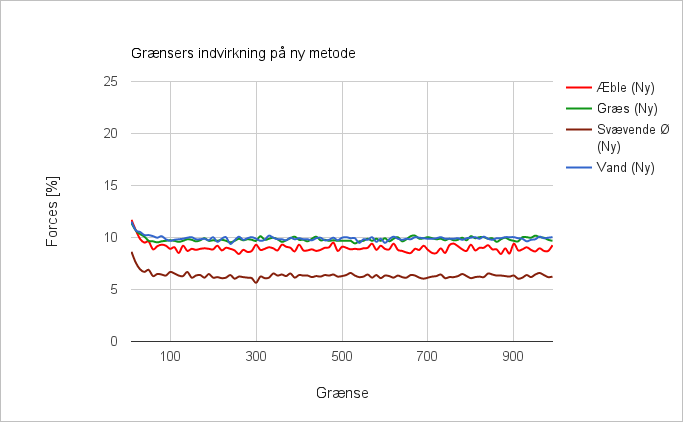
\includegraphics[width=.5\textwidth]{figures/graphNew.png}}
\caption{my caption}
\end{figure}
\end{frame}
\begin{frame}{Status}{}
\begin{figure}
\centering     %%% not \center
\subfigure[]{\label{fig:a}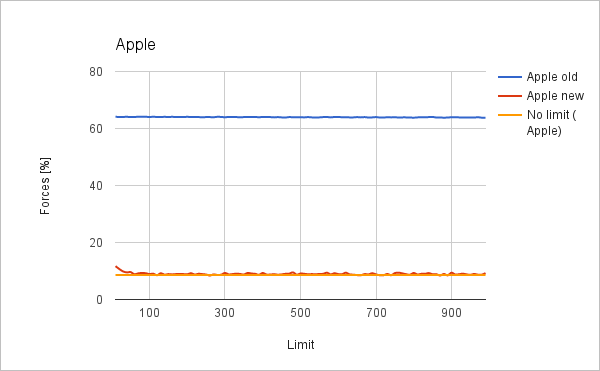
\includegraphics[width=.4\textwidth]{figures/graphApple.png}}
\subfigure[]{\label{fig:b}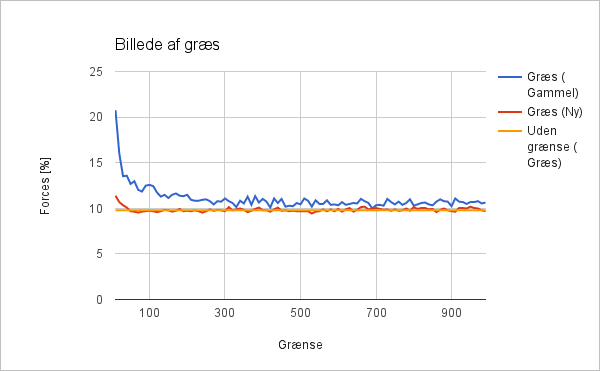
\includegraphics[width=.4\textwidth]{figures/graphGrass.png}}
\subfigure[]{\label{fig:a}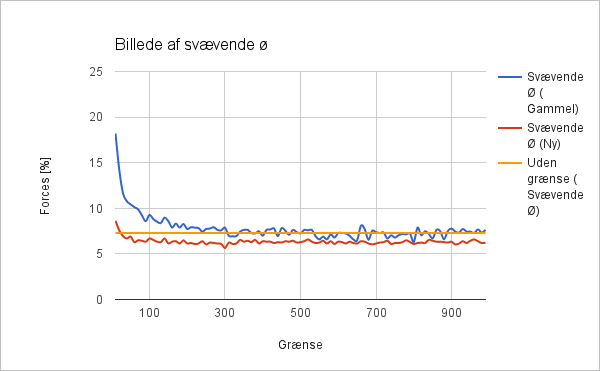
\includegraphics[width=.4\textwidth]{figures/graphIsland.png}}
\subfigure[]{\label{fig:b}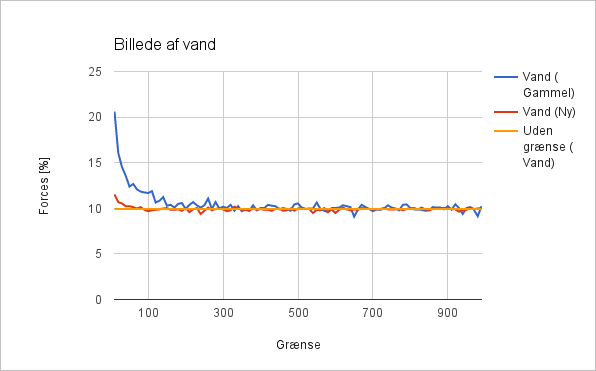
\includegraphics[width=.4\textwidth]{figures/graphWater.png}}
\caption{Sammenligning af grænseværdier}
\label{fig:limits}
\end{figure}
\end{frame}

\begin{frame}{Status}{}
\begin{figure}
\centering     %%% not \center
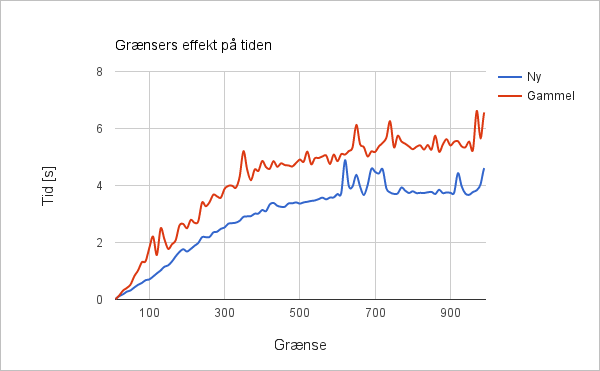
\includegraphics[width=.6\textwidth]{figures/graphTime.png}
\caption{Effekten fra grænseværdier på tiden}
\label{fig:limits}
\end{figure}
\end{frame}
   % Løsningsfase (JPEG encoder og Grafteori)
% -*- root: ../Presentation.tex -*-
\section{Optimeringer}
\begin{frame}{Optimeringer}{}
		\begin{figure}[!H]
			\centering
			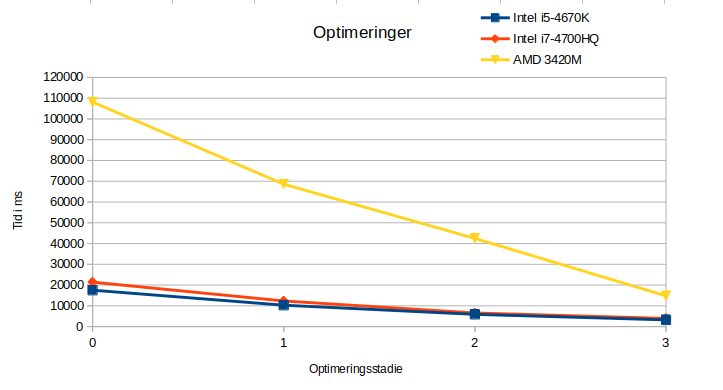
\includegraphics[width=1\textwidth]{Jacob/Selection_744.png}
	\end{figure}
\note{
	1:
	\begin{itemize}
		\item Loop logic conditions beregning flyttet ud af loop
		\item padcover image kører kun når det er nødvendigt
		\item padcoverimage bruger ikke getpixel/setpixel
	\end{itemize}

	2:
	\begin{itemize}
		\item splitToChannels bruger ikke getPixel
	\end{itemize}

	3:
	\begin{itemize}
		\item Multithreading
	\end{itemize}
}
\end{frame}
% -*- root: ../Presentation.tex -*-
\section{Programdemo}
%PNG SECTION
\begin{frame}{Programdemo}{}
	
\end{frame}
% -*- root: ../Presentation.tex -*-
\section{Forbedringer}
\begin{frame}{Forbedringer til programmet}{}
	Problemer vi ville løse:
	\begin{itemize}
		\item Primitiv tilgang til \lstinline|Graph| klassens opbygning
		\item Megen funktionalitet gemt i \lstinline|JPEGImage| klassen
	\end{itemize}
\end{frame}

\subsection{Ændringer til \lstinline|Graph|}
\begin{frame}{Ændringer til \lstinline|Graph|}{}
	3 forskellige måder at opbygge en graf:
	\begin{enumerate}
		\item Liste af Vertices og Edges\uncover<2-2>{\textcolor{red}{$\leftarrow$}}
		\item Naboliste (Adjacency List)\uncover<3-3>{\textcolor{red}{$\leftarrow$}}
		\item Nabomatrix (Adjacency Matrix)
	\end{enumerate}
\note<.-> {
	I afsnit 3.3  diskuteres forskellige fremstillinger. Vi bruger den simple, men beskriver adjancency listen som værende en god ide.

	Vi havde et ønske om at benytte den
}
\end{frame}

\begin{frame}{Fordel ved naboliste}{}

\includegraphics[width=\textwidth]{figures/graphLists.png}
\note<.-> {
	(1)
	For at slette en kant skal vi loope igennem alle vores kanter, og kun slette dem vi skal bruge.
	Resulterer i mange spildte operationer

	(2)
	Vi skal kun loope igennem de kanter der bliver peget på af edges i naboerne til en vertex
}
\end{frame}



\begin{frame}[fragile]{Svaret er...}{}
\lstinline|GraphEncoder|
\begin{itemize}
	\item Håndterer alt graf-enkodning
	\item En generel løsning fremfor specialsyet til JPEG
	\item Maksimerer data-hiding og testabilitet
\end{itemize}

\only<1-1> {
	\lstinputlisting[breaklines=true,basicstyle=\tiny,frame=single]{Mathias/code1.cs}
}
\only<2-2> {
	\lstinputlisting[breaklines=true,basicstyle=\tiny,frame=single]{Mathias/code2.cs}
}
\note<.->{
	Vi kan gemme alt graf væk fra JPEG. Det er kun grafen selv der behøver at kende til det.

	Dette betyder at løsningen kan fungere på ``alle'' tal. Ikke kun AC koefficienter. GraphEncoder er ligeglad hvor tallene kommer fra

	Vi kan gøre løsningen mere fleksibel ved hjælp af interfaces

	Forskellige typer af graffremstillinger kunne skiftes ud på runtime eller når et nyt bliver lavet
}
\end{frame}
% -*- root: ../Presentation.tex -*-
\section{Status}
\begin{frame}{Status}{}
\begin{figure}
\centering     %%% not \center
\subfigure[Grænseværdier på gamle program]{\label{fig:a}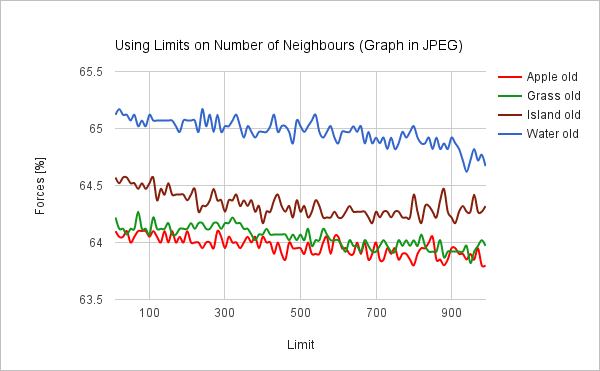
\includegraphics[width=.5\textwidth]{figures/graphOld.png}}
\subfigure[Grænseværdier på nye program]{\label{fig:b}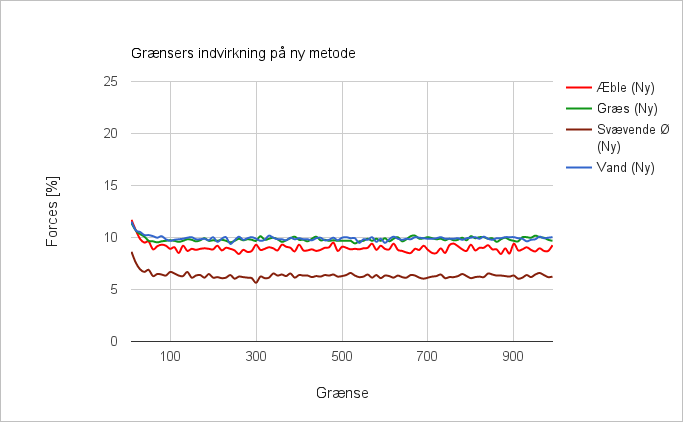
\includegraphics[width=.5\textwidth]{figures/graphNew.png}}
\caption{my caption}
\end{figure}
\end{frame}
\begin{frame}{Status}{}
\begin{figure}
\centering     %%% not \center
\subfigure[]{\label{fig:a}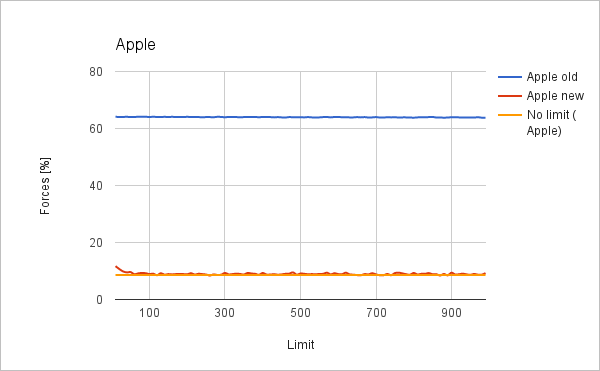
\includegraphics[width=.4\textwidth]{figures/graphApple.png}}
\subfigure[]{\label{fig:b}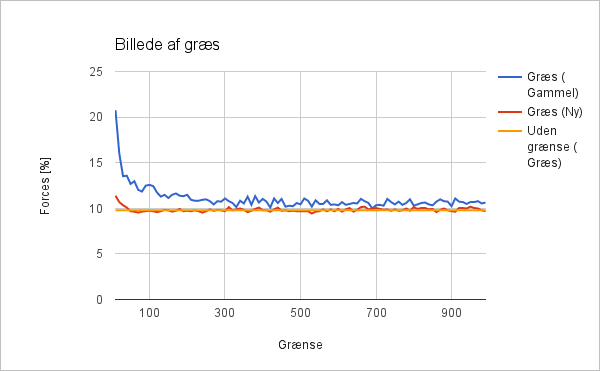
\includegraphics[width=.4\textwidth]{figures/graphGrass.png}}
\subfigure[]{\label{fig:a}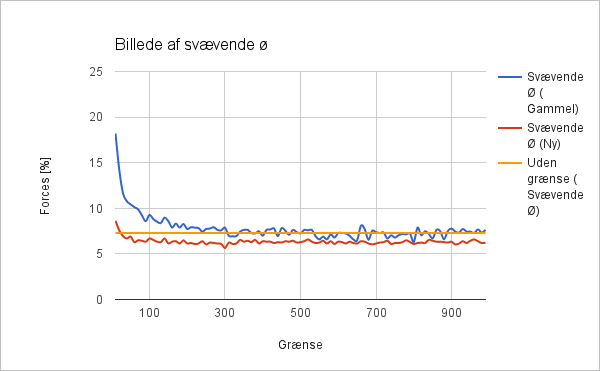
\includegraphics[width=.4\textwidth]{figures/graphIsland.png}}
\subfigure[]{\label{fig:b}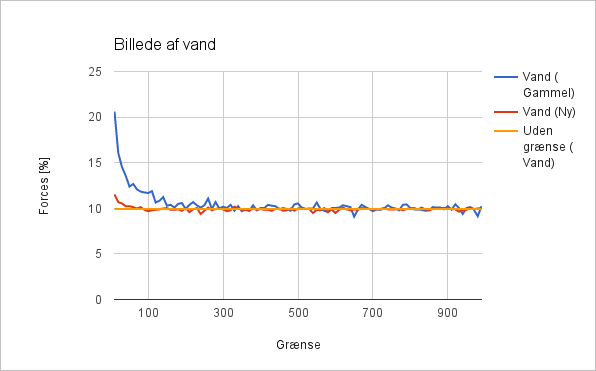
\includegraphics[width=.4\textwidth]{figures/graphWater.png}}
\caption{Sammenligning af grænseværdier}
\label{fig:limits}
\end{figure}
\end{frame}

\begin{frame}{Status}{}
\begin{figure}
\centering     %%% not \center
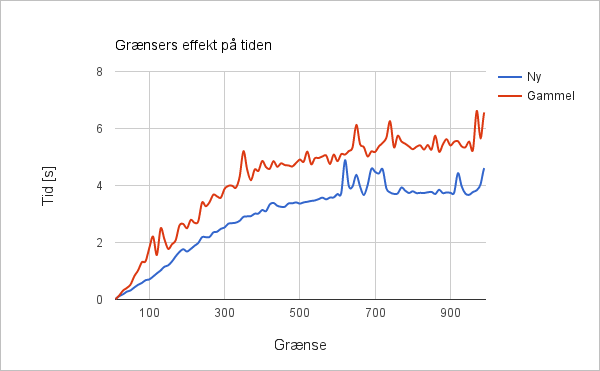
\includegraphics[width=.6\textwidth]{figures/graphTime.png}
\caption{Effekten fra grænseværdier på tiden}
\label{fig:limits}
\end{figure}
\end{frame}
    % Udvikling af encode/decode på samme tid, forklaring af encode/decode, optimering
% -*- root: ../Presentation.tex -*-
\section{Optimeringer}
\begin{frame}{Optimeringer}{}
		\begin{figure}[!H]
			\centering
			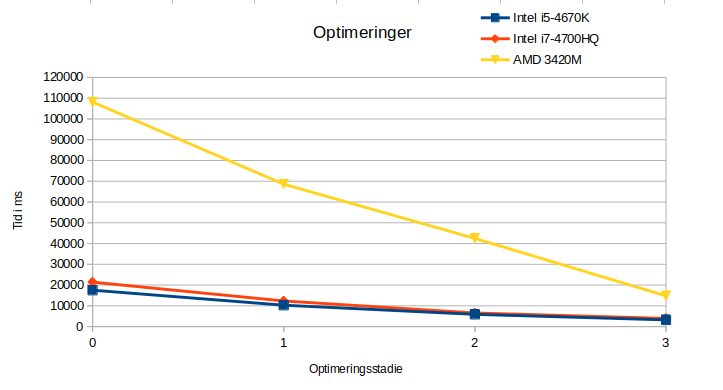
\includegraphics[width=1\textwidth]{Jacob/Selection_744.png}
	\end{figure}
\note{
	1:
	\begin{itemize}
		\item Loop logic conditions beregning flyttet ud af loop
		\item padcover image kører kun når det er nødvendigt
		\item padcoverimage bruger ikke getpixel/setpixel
	\end{itemize}

	2:
	\begin{itemize}
		\item splitToChannels bruger ikke getPixel
	\end{itemize}

	3:
	\begin{itemize}
		\item Multithreading
	\end{itemize}
}
\end{frame}
% -*- root: ../Presentation.tex -*-
\section{Programdemo}
%PNG SECTION
\begin{frame}{Programdemo}{}
	
\end{frame}
% -*- root: ../Presentation.tex -*-
\section{Forbedringer}
\begin{frame}{Forbedringer til programmet}{}
	Problemer vi ville løse:
	\begin{itemize}
		\item Primitiv tilgang til \lstinline|Graph| klassens opbygning
		\item Megen funktionalitet gemt i \lstinline|JPEGImage| klassen
	\end{itemize}
\end{frame}

\subsection{Ændringer til \lstinline|Graph|}
\begin{frame}{Ændringer til \lstinline|Graph|}{}
	3 forskellige måder at opbygge en graf:
	\begin{enumerate}
		\item Liste af Vertices og Edges\uncover<2-2>{\textcolor{red}{$\leftarrow$}}
		\item Naboliste (Adjacency List)\uncover<3-3>{\textcolor{red}{$\leftarrow$}}
		\item Nabomatrix (Adjacency Matrix)
	\end{enumerate}
\note<.-> {
	I afsnit 3.3  diskuteres forskellige fremstillinger. Vi bruger den simple, men beskriver adjancency listen som værende en god ide.

	Vi havde et ønske om at benytte den
}
\end{frame}

\begin{frame}{Fordel ved naboliste}{}

\includegraphics[width=\textwidth]{figures/graphLists.png}
\note<.-> {
	(1)
	For at slette en kant skal vi loope igennem alle vores kanter, og kun slette dem vi skal bruge.
	Resulterer i mange spildte operationer

	(2)
	Vi skal kun loope igennem de kanter der bliver peget på af edges i naboerne til en vertex
}
\end{frame}



\begin{frame}[fragile]{Svaret er...}{}
\lstinline|GraphEncoder|
\begin{itemize}
	\item Håndterer alt graf-enkodning
	\item En generel løsning fremfor specialsyet til JPEG
	\item Maksimerer data-hiding og testabilitet
\end{itemize}

\only<1-1> {
	\lstinputlisting[breaklines=true,basicstyle=\tiny,frame=single]{Mathias/code1.cs}
}
\only<2-2> {
	\lstinputlisting[breaklines=true,basicstyle=\tiny,frame=single]{Mathias/code2.cs}
}
\note<.->{
	Vi kan gemme alt graf væk fra JPEG. Det er kun grafen selv der behøver at kende til det.

	Dette betyder at løsningen kan fungere på ``alle'' tal. Ikke kun AC koefficienter. GraphEncoder er ligeglad hvor tallene kommer fra

	Vi kan gøre løsningen mere fleksibel ved hjælp af interfaces

	Forskellige typer af graffremstillinger kunne skiftes ud på runtime eller når et nyt bliver lavet
}
\end{frame}
% -*- root: ../Presentation.tex -*-
\section{Status}
\begin{frame}{Status}{}
\begin{figure}
\centering     %%% not \center
\subfigure[Grænseværdier på gamle program]{\label{fig:a}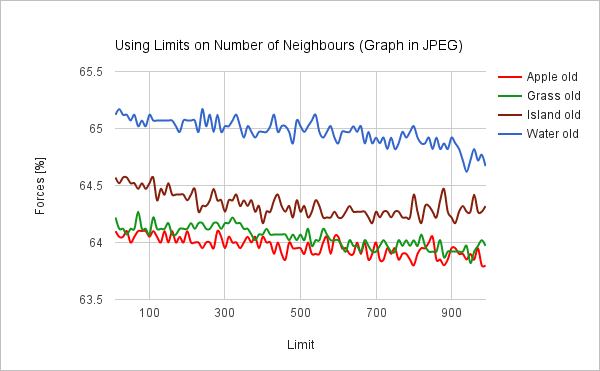
\includegraphics[width=.5\textwidth]{figures/graphOld.png}}
\subfigure[Grænseværdier på nye program]{\label{fig:b}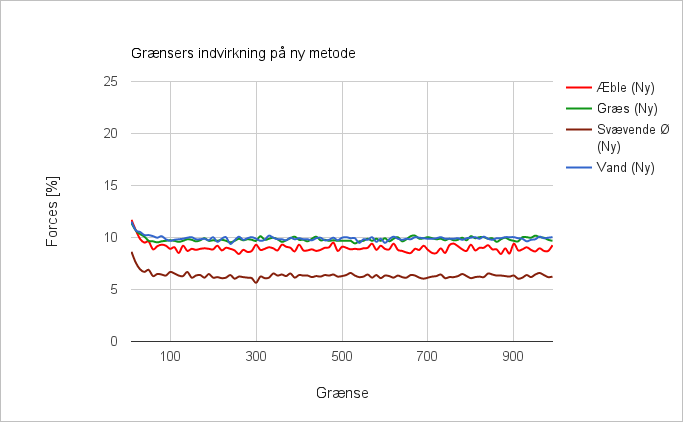
\includegraphics[width=.5\textwidth]{figures/graphNew.png}}
\caption{my caption}
\end{figure}
\end{frame}
\begin{frame}{Status}{}
\begin{figure}
\centering     %%% not \center
\subfigure[]{\label{fig:a}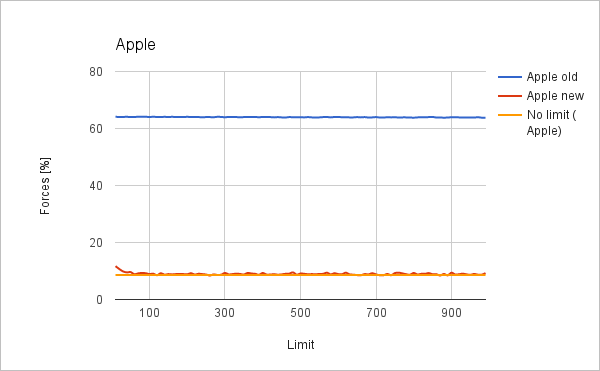
\includegraphics[width=.4\textwidth]{figures/graphApple.png}}
\subfigure[]{\label{fig:b}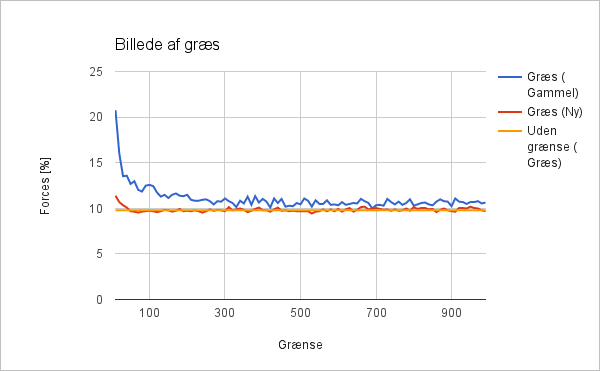
\includegraphics[width=.4\textwidth]{figures/graphGrass.png}}
\subfigure[]{\label{fig:a}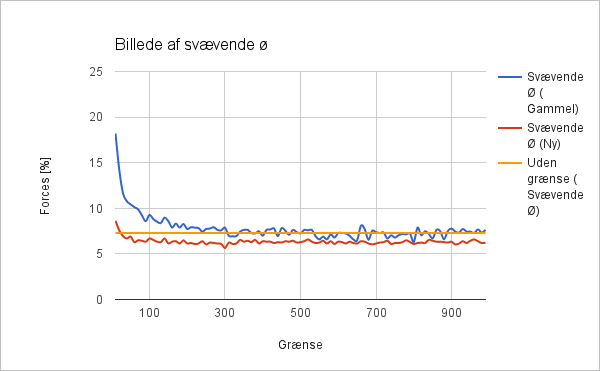
\includegraphics[width=.4\textwidth]{figures/graphIsland.png}}
\subfigure[]{\label{fig:b}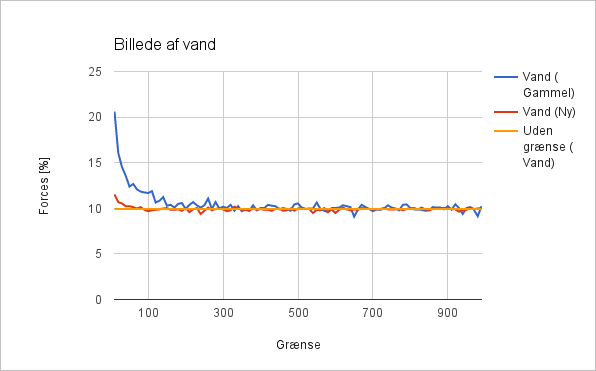
\includegraphics[width=.4\textwidth]{figures/graphWater.png}}
\caption{Sammenligning af grænseværdier}
\label{fig:limits}
\end{figure}
\end{frame}

\begin{frame}{Status}{}
\begin{figure}
\centering     %%% not \center
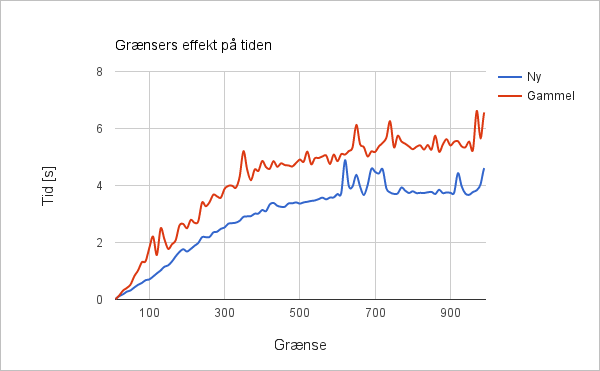
\includegraphics[width=.6\textwidth]{figures/graphTime.png}
\caption{Effekten fra grænseværdier på tiden}
\label{fig:limits}
\end{figure}
\end{frame}
  % programdemo, forbedring af graf, status af program
% -*- root: ../Presentation.tex -*-
\section{Optimeringer}
\begin{frame}{Optimeringer}{}
		\begin{figure}[!H]
			\centering
			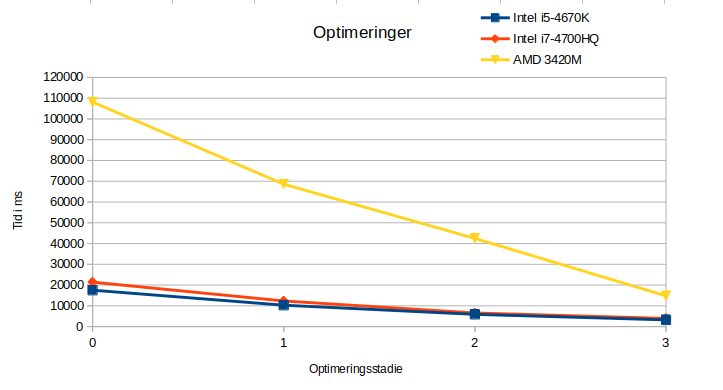
\includegraphics[width=1\textwidth]{Jacob/Selection_744.png}
	\end{figure}
\note{
	1:
	\begin{itemize}
		\item Loop logic conditions beregning flyttet ud af loop
		\item padcover image kører kun når det er nødvendigt
		\item padcoverimage bruger ikke getpixel/setpixel
	\end{itemize}

	2:
	\begin{itemize}
		\item splitToChannels bruger ikke getPixel
	\end{itemize}

	3:
	\begin{itemize}
		\item Multithreading
	\end{itemize}
}
\end{frame}
% -*- root: ../Presentation.tex -*-
\section{Programdemo}
%PNG SECTION
\begin{frame}{Programdemo}{}
	
\end{frame}
% -*- root: ../Presentation.tex -*-
\section{Forbedringer}
\begin{frame}{Forbedringer til programmet}{}
	Problemer vi ville løse:
	\begin{itemize}
		\item Primitiv tilgang til \lstinline|Graph| klassens opbygning
		\item Megen funktionalitet gemt i \lstinline|JPEGImage| klassen
	\end{itemize}
\end{frame}

\subsection{Ændringer til \lstinline|Graph|}
\begin{frame}{Ændringer til \lstinline|Graph|}{}
	3 forskellige måder at opbygge en graf:
	\begin{enumerate}
		\item Liste af Vertices og Edges\uncover<2-2>{\textcolor{red}{$\leftarrow$}}
		\item Naboliste (Adjacency List)\uncover<3-3>{\textcolor{red}{$\leftarrow$}}
		\item Nabomatrix (Adjacency Matrix)
	\end{enumerate}
\note<.-> {
	I afsnit 3.3  diskuteres forskellige fremstillinger. Vi bruger den simple, men beskriver adjancency listen som værende en god ide.

	Vi havde et ønske om at benytte den
}
\end{frame}

\begin{frame}{Fordel ved naboliste}{}

\includegraphics[width=\textwidth]{figures/graphLists.png}
\note<.-> {
	(1)
	For at slette en kant skal vi loope igennem alle vores kanter, og kun slette dem vi skal bruge.
	Resulterer i mange spildte operationer

	(2)
	Vi skal kun loope igennem de kanter der bliver peget på af edges i naboerne til en vertex
}
\end{frame}



\begin{frame}[fragile]{Svaret er...}{}
\lstinline|GraphEncoder|
\begin{itemize}
	\item Håndterer alt graf-enkodning
	\item En generel løsning fremfor specialsyet til JPEG
	\item Maksimerer data-hiding og testabilitet
\end{itemize}

\only<1-1> {
	\lstinputlisting[breaklines=true,basicstyle=\tiny,frame=single]{Mathias/code1.cs}
}
\only<2-2> {
	\lstinputlisting[breaklines=true,basicstyle=\tiny,frame=single]{Mathias/code2.cs}
}
\note<.->{
	Vi kan gemme alt graf væk fra JPEG. Det er kun grafen selv der behøver at kende til det.

	Dette betyder at løsningen kan fungere på ``alle'' tal. Ikke kun AC koefficienter. GraphEncoder er ligeglad hvor tallene kommer fra

	Vi kan gøre løsningen mere fleksibel ved hjælp af interfaces

	Forskellige typer af graffremstillinger kunne skiftes ud på runtime eller når et nyt bliver lavet
}
\end{frame}
% -*- root: ../Presentation.tex -*-
\section{Status}
\begin{frame}{Status}{}
\begin{figure}
\centering     %%% not \center
\subfigure[Grænseværdier på gamle program]{\label{fig:a}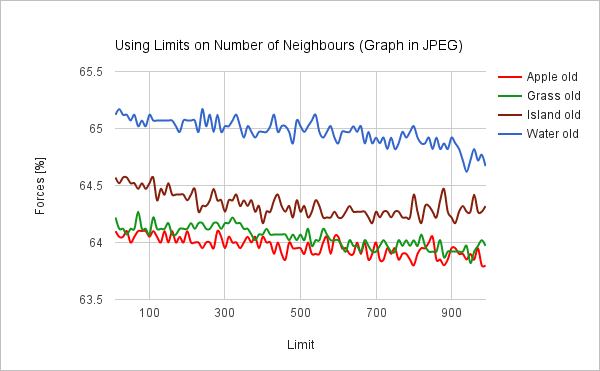
\includegraphics[width=.5\textwidth]{figures/graphOld.png}}
\subfigure[Grænseværdier på nye program]{\label{fig:b}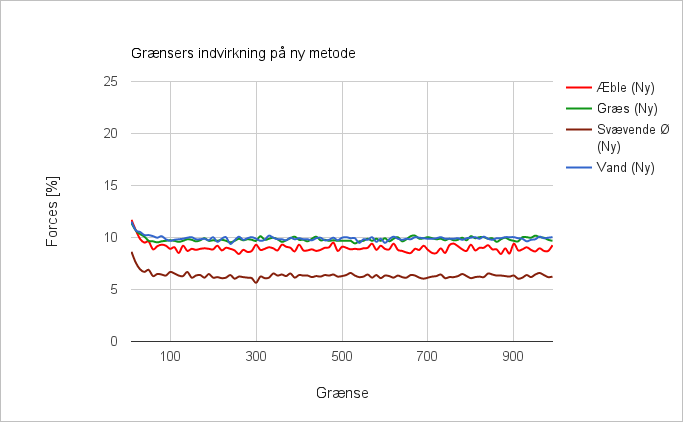
\includegraphics[width=.5\textwidth]{figures/graphNew.png}}
\caption{my caption}
\end{figure}
\end{frame}
\begin{frame}{Status}{}
\begin{figure}
\centering     %%% not \center
\subfigure[]{\label{fig:a}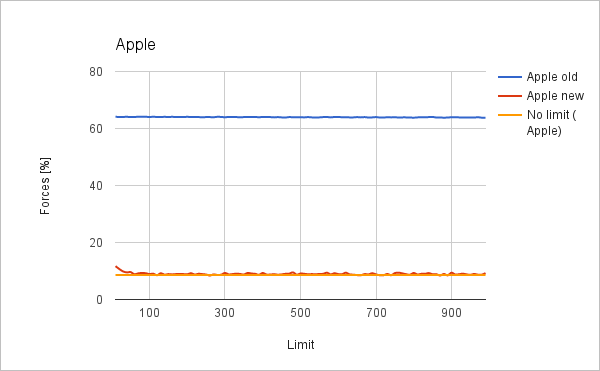
\includegraphics[width=.4\textwidth]{figures/graphApple.png}}
\subfigure[]{\label{fig:b}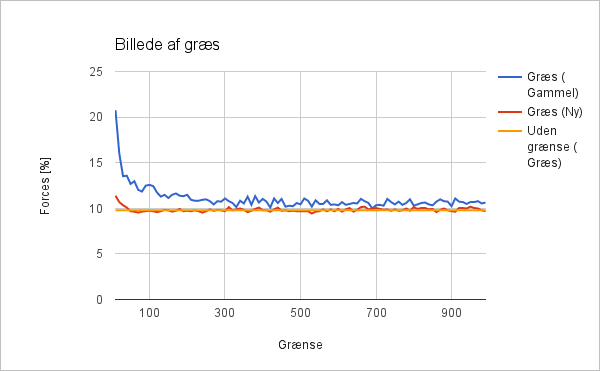
\includegraphics[width=.4\textwidth]{figures/graphGrass.png}}
\subfigure[]{\label{fig:a}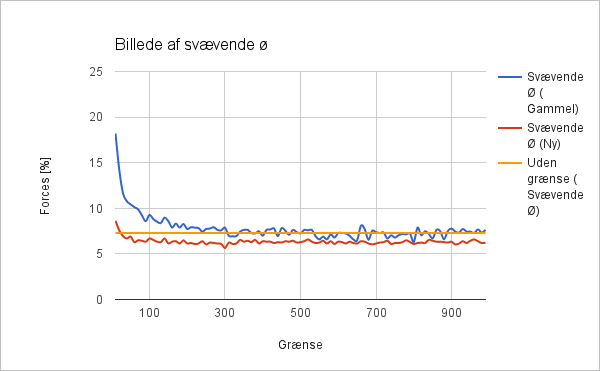
\includegraphics[width=.4\textwidth]{figures/graphIsland.png}}
\subfigure[]{\label{fig:b}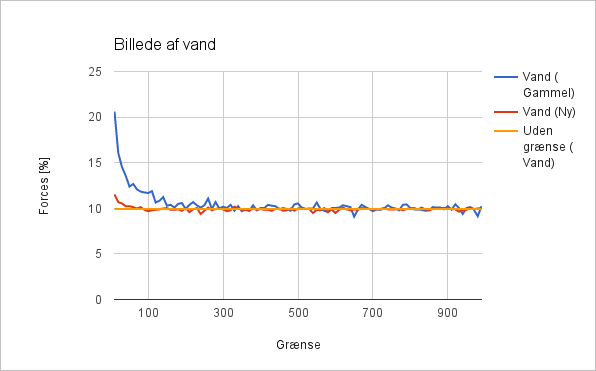
\includegraphics[width=.4\textwidth]{figures/graphWater.png}}
\caption{Sammenligning af grænseværdier}
\label{fig:limits}
\end{figure}
\end{frame}

\begin{frame}{Status}{}
\begin{figure}
\centering     %%% not \center
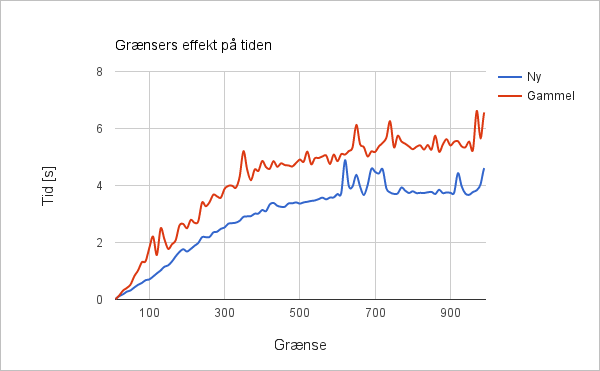
\includegraphics[width=.6\textwidth]{figures/graphTime.png}
\caption{Effekten fra grænseværdier på tiden}
\label{fig:limits}
\end{figure}
\end{frame}
      % Steganalysis
% -*- root: ../Presentation.tex -*-
\section{Optimeringer}
\begin{frame}{Optimeringer}{}
		\begin{figure}[!H]
			\centering
			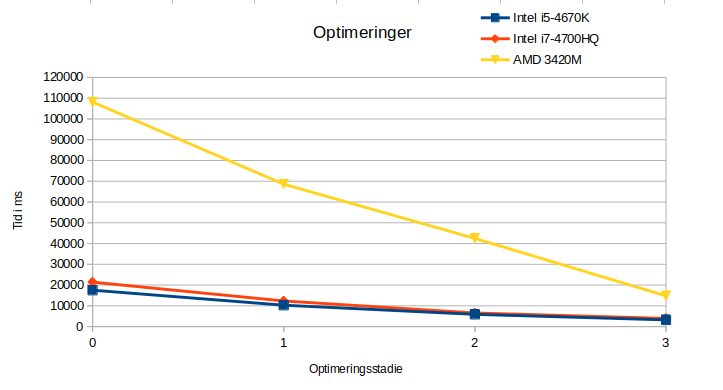
\includegraphics[width=1\textwidth]{Jacob/Selection_744.png}
	\end{figure}
\note{
	1:
	\begin{itemize}
		\item Loop logic conditions beregning flyttet ud af loop
		\item padcover image kører kun når det er nødvendigt
		\item padcoverimage bruger ikke getpixel/setpixel
	\end{itemize}

	2:
	\begin{itemize}
		\item splitToChannels bruger ikke getPixel
	\end{itemize}

	3:
	\begin{itemize}
		\item Multithreading
	\end{itemize}
}
\end{frame}
% -*- root: ../Presentation.tex -*-
\section{Programdemo}
%PNG SECTION
\begin{frame}{Programdemo}{}
	
\end{frame}
% -*- root: ../Presentation.tex -*-
\section{Forbedringer}
\begin{frame}{Forbedringer til programmet}{}
	Problemer vi ville løse:
	\begin{itemize}
		\item Primitiv tilgang til \lstinline|Graph| klassens opbygning
		\item Megen funktionalitet gemt i \lstinline|JPEGImage| klassen
	\end{itemize}
\end{frame}

\subsection{Ændringer til \lstinline|Graph|}
\begin{frame}{Ændringer til \lstinline|Graph|}{}
	3 forskellige måder at opbygge en graf:
	\begin{enumerate}
		\item Liste af Vertices og Edges\uncover<2-2>{\textcolor{red}{$\leftarrow$}}
		\item Naboliste (Adjacency List)\uncover<3-3>{\textcolor{red}{$\leftarrow$}}
		\item Nabomatrix (Adjacency Matrix)
	\end{enumerate}
\note<.-> {
	I afsnit 3.3  diskuteres forskellige fremstillinger. Vi bruger den simple, men beskriver adjancency listen som værende en god ide.

	Vi havde et ønske om at benytte den
}
\end{frame}

\begin{frame}{Fordel ved naboliste}{}

\includegraphics[width=\textwidth]{figures/graphLists.png}
\note<.-> {
	(1)
	For at slette en kant skal vi loope igennem alle vores kanter, og kun slette dem vi skal bruge.
	Resulterer i mange spildte operationer

	(2)
	Vi skal kun loope igennem de kanter der bliver peget på af edges i naboerne til en vertex
}
\end{frame}



\begin{frame}[fragile]{Svaret er...}{}
\lstinline|GraphEncoder|
\begin{itemize}
	\item Håndterer alt graf-enkodning
	\item En generel løsning fremfor specialsyet til JPEG
	\item Maksimerer data-hiding og testabilitet
\end{itemize}

\only<1-1> {
	\lstinputlisting[breaklines=true,basicstyle=\tiny,frame=single]{Mathias/code1.cs}
}
\only<2-2> {
	\lstinputlisting[breaklines=true,basicstyle=\tiny,frame=single]{Mathias/code2.cs}
}
\note<.->{
	Vi kan gemme alt graf væk fra JPEG. Det er kun grafen selv der behøver at kende til det.

	Dette betyder at løsningen kan fungere på ``alle'' tal. Ikke kun AC koefficienter. GraphEncoder er ligeglad hvor tallene kommer fra

	Vi kan gøre løsningen mere fleksibel ved hjælp af interfaces

	Forskellige typer af graffremstillinger kunne skiftes ud på runtime eller når et nyt bliver lavet
}
\end{frame}
% -*- root: ../Presentation.tex -*-
\section{Status}
\begin{frame}{Status}{}
\begin{figure}
\centering     %%% not \center
\subfigure[Grænseværdier på gamle program]{\label{fig:a}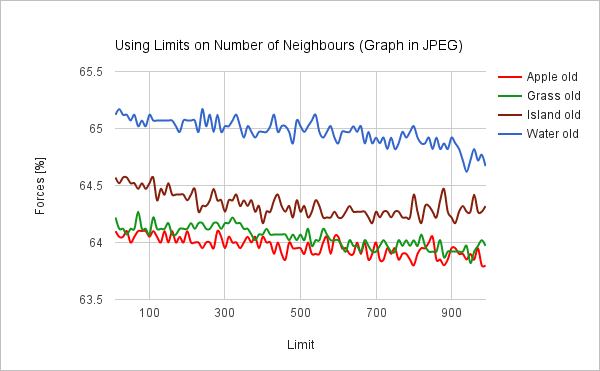
\includegraphics[width=.5\textwidth]{figures/graphOld.png}}
\subfigure[Grænseværdier på nye program]{\label{fig:b}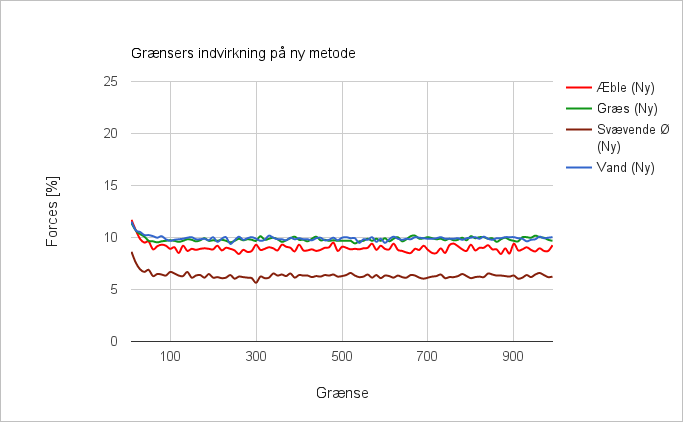
\includegraphics[width=.5\textwidth]{figures/graphNew.png}}
\caption{my caption}
\end{figure}
\end{frame}
\begin{frame}{Status}{}
\begin{figure}
\centering     %%% not \center
\subfigure[]{\label{fig:a}\includegraphics[width=.4\textwidth]{figures/graphApple.png}}
\subfigure[]{\label{fig:b}\includegraphics[width=.4\textwidth]{figures/graphGrass.png}}
\subfigure[]{\label{fig:a}\includegraphics[width=.4\textwidth]{figures/graphIsland.png}}
\subfigure[]{\label{fig:b}\includegraphics[width=.4\textwidth]{figures/graphWater.png}}
\caption{Sammenligning af grænseværdier}
\label{fig:limits}
\end{figure}
\end{frame}

\begin{frame}{Status}{}
\begin{figure}
\centering     %%% not \center
\includegraphics[width=.6\textwidth]{figures/graphTime.png}
\caption{Effekten fra grænseværdier på tiden}
\label{fig:limits}
\end{figure}
\end{frame}
    % Diskussion (+ testabilitet), konklusion
% -*- root: ../Presentation.tex -*-
\section{Optimeringer}
\begin{frame}{Optimeringer}{}
		\begin{figure}[!H]
			\centering
			\includegraphics[width=1\textwidth]{Jacob/Selection_744.png}
	\end{figure}
\note{
	1:
	\begin{itemize}
		\item Loop logic conditions beregning flyttet ud af loop
		\item padcover image kører kun når det er nødvendigt
		\item padcoverimage bruger ikke getpixel/setpixel
	\end{itemize}

	2:
	\begin{itemize}
		\item splitToChannels bruger ikke getPixel
	\end{itemize}

	3:
	\begin{itemize}
		\item Multithreading
	\end{itemize}
}
\end{frame}
% -*- root: ../Presentation.tex -*-
\section{Programdemo}
%PNG SECTION
\begin{frame}{Programdemo}{}
	
\end{frame}
% -*- root: ../Presentation.tex -*-
\section{Forbedringer}
\begin{frame}{Forbedringer til programmet}{}
	Problemer vi ville løse:
	\begin{itemize}
		\item Primitiv tilgang til \lstinline|Graph| klassens opbygning
		\item Megen funktionalitet gemt i \lstinline|JPEGImage| klassen
	\end{itemize}
\end{frame}

\subsection{Ændringer til \lstinline|Graph|}
\begin{frame}{Ændringer til \lstinline|Graph|}{}
	3 forskellige måder at opbygge en graf:
	\begin{enumerate}
		\item Liste af Vertices og Edges\uncover<2-2>{\textcolor{red}{$\leftarrow$}}
		\item Naboliste (Adjacency List)\uncover<3-3>{\textcolor{red}{$\leftarrow$}}
		\item Nabomatrix (Adjacency Matrix)
	\end{enumerate}
\note<.-> {
	I afsnit 3.3  diskuteres forskellige fremstillinger. Vi bruger den simple, men beskriver adjancency listen som værende en god ide.

	Vi havde et ønske om at benytte den
}
\end{frame}

\begin{frame}{Fordel ved naboliste}{}
\includegraphics[width=\textwidth]{figures/graphLists.png}
\note<.-> {
	(1)
	For at slette en kant skal vi loope igennem alle vores kanter, og kun slette dem vi skal bruge.
	Resulterer i mange spildte operationer

	(2)
	Vi skal kun loope igennem de kanter der bliver peget på af edges i naboerne til en vertex
}
\end{frame}



\begin{frame}[fragile]{Svaret er...}{}
\lstinline|GraphEncoder|
\begin{itemize}
	\item Håndterer alt graf-enkodning
	\item En generel løsning fremfor specialsyet til JPEG
	\item Maksimerer data-hiding og testabilitet
\end{itemize}

\only<1-1> {
	\lstinputlisting[breaklines=true,basicstyle=\tiny,frame=single]{Mathias/code1.cs}
}
\only<2-2> {
	\lstinputlisting[breaklines=true,basicstyle=\tiny,frame=single]{Mathias/code2.cs}
}
\note<.->{
	Vi kan gemme alt graf væk fra JPEG. Det er kun grafen selv der behøver at kende til det.

	Dette betyder at løsningen kan fungere på ``alle'' tal. Ikke kun AC koefficienter. GraphEncoder er ligeglad hvor tallene kommer fra

	Vi kan gøre løsningen mere fleksibel ved hjælp af interfaces

	Forskellige typer af graffremstillinger kunne skiftes ud på runtime eller når et nyt bliver lavet
}
\end{frame}
% -*- root: ../Presentation.tex -*-
\section{Status}
\begin{frame}{Status}{}
\begin{figure}
\centering     %%% not \center
\subfigure[Grænseværdier på gamle program]{\label{fig:a}\includegraphics[width=.5\textwidth]{figures/graphOld.png}}
\subfigure[Grænseværdier på nye program]{\label{fig:b}\includegraphics[width=.5\textwidth]{figures/graphNew.png}}
\caption{my caption}
\end{figure}
\end{frame}
\begin{frame}{Status}{}
\begin{figure}
\centering     %%% not \center
\subfigure[]{\label{fig:a}\includegraphics[width=.4\textwidth]{figures/graphApple.png}}
\subfigure[]{\label{fig:b}\includegraphics[width=.4\textwidth]{figures/graphGrass.png}}
\subfigure[]{\label{fig:a}\includegraphics[width=.4\textwidth]{figures/graphIsland.png}}
\subfigure[]{\label{fig:b}\includegraphics[width=.4\textwidth]{figures/graphWater.png}}
\caption{Sammenligning af grænseværdier}
\label{fig:limits}
\end{figure}
\end{frame}

\begin{frame}{Status}{}
\begin{figure}
\centering     %%% not \center
\includegraphics[width=.6\textwidth]{figures/graphTime.png}
\caption{Effekten fra grænseværdier på tiden}
\label{fig:limits}
\end{figure}
\end{frame}
   % Procesanalyse

{\aauwavesbg
\begin{frame}[plain,noframenumbering]
  \finalpage{DAT2-423}
\end{frame}}
%%%%%%%%%%%%%%%%

\end{document}
